\documentclass[6pt]{beamer}
\usepackage[english]{babel}
\usepackage{graphicx}
\usepackage{multimedia}
\usepackage{hyperref}
\usepackage{subfigure}
\usepackage[english]{babel}
\usepackage{booktabs}
\usepackage{tabularx}
\usepackage[utf8]{inputenc}
\usepackage[T1]{fontenc}
\usepackage{textpos}
\usepackage{lmodern}
\usepackage{xcoffins}
\usepackage{comment}
\usepackage{algorithmic}
\newcommand{\putat}[3]{\begin{picture}(0,0)(0,0)\put(#1,#2){#3}\end{picture}}
\usetheme{bjeldbak}
\usepackage[backend=biber,style=authortitle]{biblatex}
\addbibresource{Bibliography.bib}
\NewCoffin\tablecoffin
\NewDocumentCommand\Vcentre{m}
{
    \SetHorizontalCoffin\tablecoffin{#1}%
    \TypesetCoffin\tablecoffin[l,vc]%
}
  
\usepackage{mathptmx}

\renewcommand{\footnotesize}{\fontsize{4.5}{4}}

\begin{document}

\definecolor{light-gray}{gray}{0.95}
{
\usebackgroundtemplate{\putat{10}{-110}{
\includegraphics[width=0.3\paperwidth]{../Figures/Misc/ACT_logo.eps}}}
\begin{frame}[plain]
\vspace{1cm}
\begin{center}

\includegraphics[height=.07\textwidth]{../Figures/Misc/University_of_Amsterdam_logo.pdf}\\
\textsc{University} of \textsc{Amsterdam}\\ \vspace{0.2cm}
\rule{\textwidth}{1pt}\\
{\Large Evolution of Soft Robots by\\ Novelty Search}\\[0.2cm] % Thesis title
\rule{\textwidth}{0.5pt}\\ \vspace{0.4cm}
\begin{minipage}[t][1cm][t]{0,49\textwidth}
\small
\begin{flushleft}
{\scriptsize \emph{ By:}}\\
Georgios \textsc{Methenitis}
\end{flushleft}
\end{minipage}
\begin{minipage}[t][1cm][t]{0,49\textwidth}
\begin{flushright}
{\scriptsize \emph{Supervisors:}} \\
Arnaud \textsc{Visser}, {\scriptsize UvA}\\
Dario \textsc{Izzo}, {\scriptsize ESA}\\
Daniel \textsc{Hennes}, {\scriptsize ESA}
\end{flushright}
\end{minipage}\\[0.5cm]
\end{center}
\end{frame}
}

\begin{frame}
\frametitle{Outline}
\tableofcontents
\end{frame}





\section{Background}

\begin{frame}{{\scriptsize Evolution of} Soft Robots {\scriptsize by Novelty Search}}
\begin{block}{Soft Robots}
\begin{itemize}
\item Early research stage
\item Inspired by nature
\item Completely soft bodies
\item New kinds of locomotion
\end{itemize}
\end{block}
\begin{center}
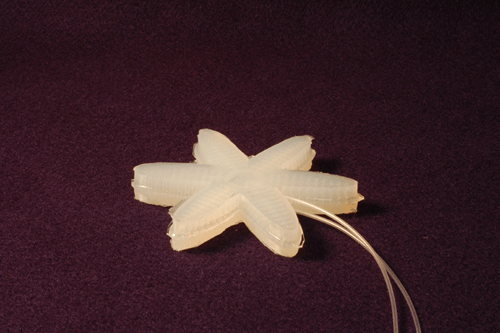
\includegraphics[width=0.3\textwidth,height=0.25\textheight]{../Figures/Misc/soft_robotics_figure.png}\		
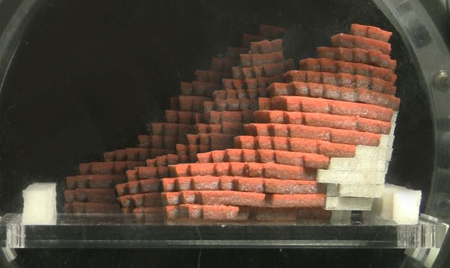
\includegraphics[width=0.3\textwidth,height=0.25\textheight]{../Figures/Misc/hillerPressureChamber.png}\	
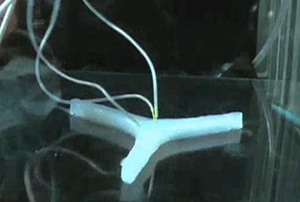
\includegraphics[width=0.3\textwidth,height=0.25\textheight]{../Figures/Misc/ExplodingRobot.jpg}\\
\end{center}
Locomotion can be achieved by pneumatic, passive, and other forms of actuation.
\end{frame}

{
\setbeamercolor{block body}{bg=white}

\begin{frame}{Evolution {\scriptsize of Soft Robots by Novelty Search}}
\begin{block}{Evolutionary algorithms}
\begin{center}
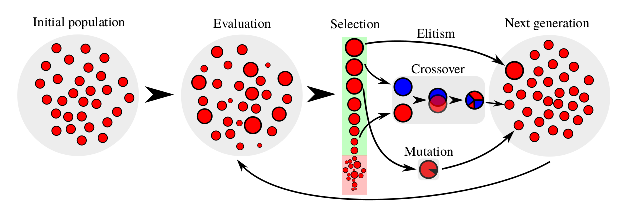
\includegraphics[width=1.0\textwidth]{../Figures/Misc/Evolution.eps}
\end{center}
\end{block}
\end{frame}

\begin{frame}{Encoding Schemes}
\begin{block}{Direct Encoding}
\begin{center}
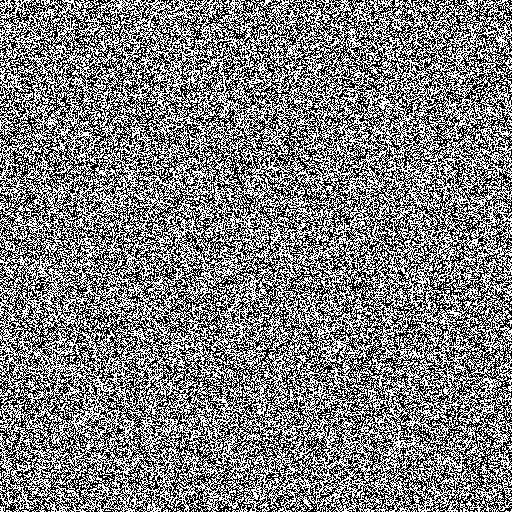
\includegraphics[width=0.4\textwidth]{../Figures/Misc/direct.jpg}
\end{center}
\end{block}
\centering
$\underbrace{010101\ldots111101}_\text{number of pixels}$
\end{frame}

\begin{frame}{Encoding Schemes}
\begin{block}{Indirect or Generative Encoding}
\begin{center}
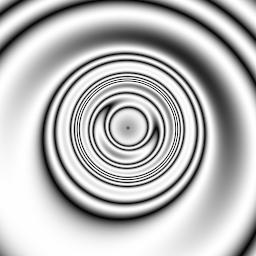
\includegraphics[width=0.4\textwidth]{../Figures/Misc/picBreed1.jpg}
\end{center}
\end{block}
\centering
$f(\underbrace{x\   ,\  y}_\text{coords.}) = \text{pixel value}$
\end{frame}
}


\begin{frame}{Compositional pattern-producing network~\footfullcite{stanley2007compositional}}
\begin{itemize}
\item Similar to artificial neural networks
\item Large set of canonical activation functions
\begin{figure}
\begin{center}
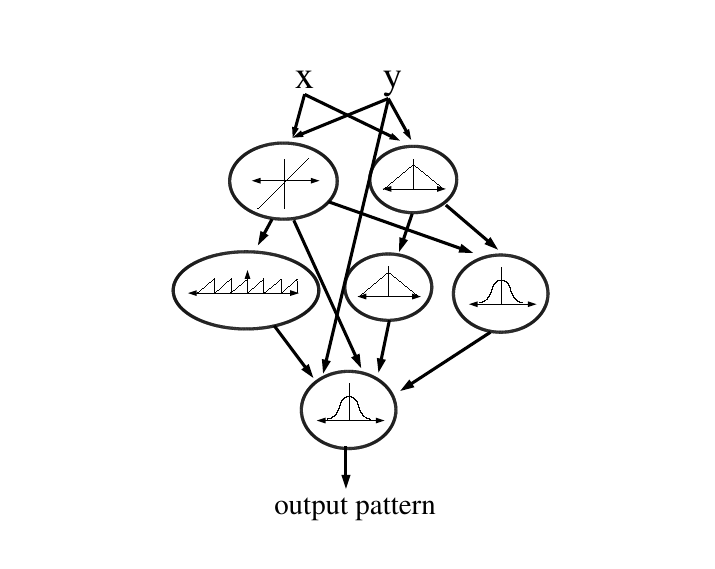
\includegraphics[scale=0.25]{../Figures/Misc/cppnNetwork.png}
\end{center}
\end{figure}
\item Produce symmetrical and repetitive patterns
\item Appropriate for problems with geometrical structure
\end{itemize}
\end{frame}

\begin{frame}{Neuroevolution}
\begin{block}{Representation of the genome}
\centering
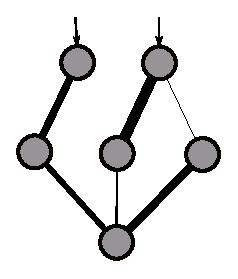
\includegraphics[height=0.7\textheight]{../Figures/Misc/networksMutationWeights1.eps}
\end{block}
\end{frame}

\begin{frame}{Neuroevolution}
\begin{block}{Traditional neuroevolution methods}
\centering
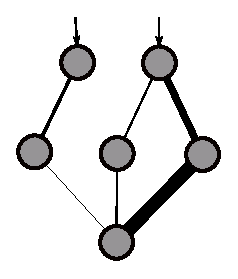
\includegraphics[height=0.7\textheight]{../Figures/Misc/networksMutationWeights2.eps}
\end{block}
\end{frame}

\begin{frame}{Neuroevolution}
\begin{block}{Adding a link}
\centering
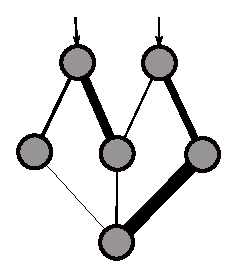
\includegraphics[height=0.7\textheight]{../Figures/Misc/networksMutationWeights3.eps}
\end{block}
\end{frame}

\begin{frame}{Neuroevolution}
\begin{block}{Adding a node}
\centering
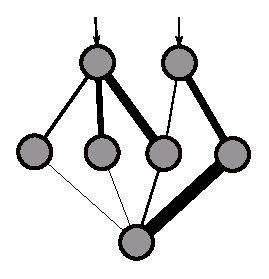
\includegraphics[height=0.7\textheight]{../Figures/Misc/networksMutationWeights4.eps}
\end{block}
\end{frame}

\begin{frame}{NeuroEvolution of Augmented Topologies (NEAT)~\footfullcite{stanley2002evolving}}
\begin{block}{Some key points of this method are:}
\begin{itemize}
\item Evolving neural network topologies along with weights
\item Crossover between different topologies
\item Structural innovation through speciation
\end{itemize}
\end{block}
\pause
\begin{block}{Genetic Operations in NEAT:}
\centering
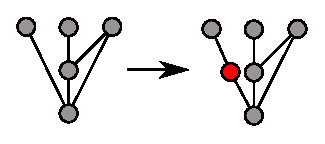
\includegraphics[height=0.25\textheight]{../Figures/Misc/neatAddNode.eps}
\end{block}
\end{frame}

\begin{frame}{NeuroEvolution of Augmented Topologies (NEAT)~\footfullcite{stanley2002evolving}}
\begin{block}{Some key points of this method are:}
\begin{itemize}
\item Evolving neural network topologies along with weights
\item Crossover between different topologies
\item Structural innovation through speciation
\end{itemize}
\end{block}
\begin{block}{Genetic Operations in NEAT:}
\centering
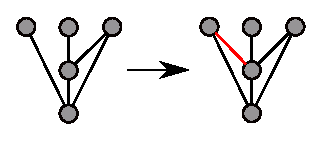
\includegraphics[height=0.25\textheight]{../Figures/Misc/neatAddLink.eps}
\end{block}
\end{frame}

\begin{frame}{NeuroEvolution of Augmented Topologies (NEAT)~\footfullcite{stanley2002evolving}}
\begin{block}{Some key points of this method are:}
\begin{itemize}
\item Evolving neural network topologies along with weights
\item Crossover between different topologies
\item Structural innovation through speciation
\end{itemize}
\end{block}
\begin{block}{Genetic Operations in NEAT:}
\centering
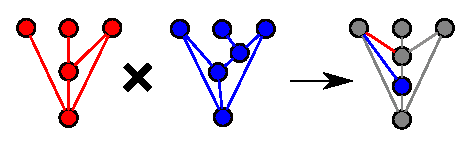
\includegraphics[height=0.25\textheight]{../Figures/Misc/neatCrossOver.eps}
\end{block}
\end{frame}

\begin{frame}{{\scriptsize Evolution of Soft Robots by} Novelty Search}
\begin{center}
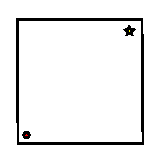
\includegraphics[width=0.55\textwidth]{../Figures/Misc/mazeEasy.eps}
\end{center}
\end{frame}

\begin{frame}{{\scriptsize Evolution of Soft Robots by} Novelty Search}
\begin{center}
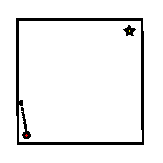
\includegraphics[width=0.55\textwidth]{../Figures/Misc/mazeEasy1.eps}
\end{center}
\end{frame}

\begin{frame}{{\scriptsize Evolution of Soft Robots by} Novelty Search}
\begin{center}
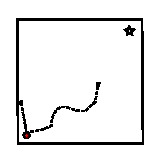
\includegraphics[width=0.55\textwidth]{../Figures/Misc/mazeEasy2.eps}
\end{center}
\end{frame}

\begin{frame}{{\scriptsize Evolution of Soft Robots by} Novelty Search}
\begin{center}
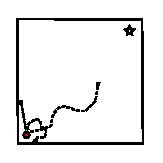
\includegraphics[width=0.55\textwidth]{../Figures/Misc/mazeEasy3.eps}
\end{center}
\end{frame}

\begin{frame}{{\scriptsize Evolution of Soft Robots by} Novelty Search}
\begin{center}
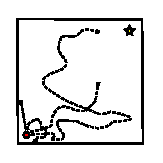
\includegraphics[width=0.55\textwidth]{../Figures/Misc/mazeEasy4.eps}
\end{center}
\end{frame}

\begin{frame}{{\scriptsize Evolution of Soft Robots by} Novelty Search}
\begin{center}
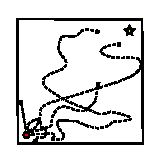
\includegraphics[width=0.55\textwidth]{../Figures/Misc/mazeEasy5.eps}
\end{center}
\end{frame}

\begin{frame}{{\scriptsize Evolution of Soft Robots by} Novelty Search}
\begin{center}
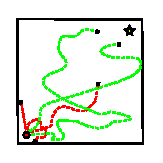
\includegraphics[width=0.55\textwidth]{../Figures/Misc/mazeEasy6.eps}
\end{center}
\end{frame}

\begin{frame}{{\scriptsize Evolution of Soft Robots by} Novelty Search}
\begin{center}
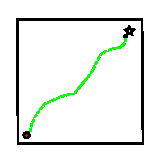
\includegraphics[width=0.55\textwidth]{../Figures/Misc/mazeEasy7.eps}
\end{center}
\end{frame}

\begin{frame}{{\scriptsize Evolution of Soft Robots by} Novelty Search}
\begin{center}

\includegraphics[width=0.55\textwidth]{../Figures/Misc/maze.eps}
\end{center}
\end{frame}

\begin{frame}{{\scriptsize Evolution of Soft Robots by} Novelty Search}
\begin{center}

\includegraphics[width=0.55\textwidth]{../Figures/Misc/maze1.eps}
\end{center}
\end{frame}

\begin{frame}{{\scriptsize Evolution of Soft Robots by} Novelty Search}
\begin{center}
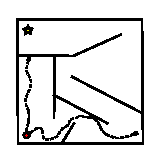
\includegraphics[width=0.55\textwidth]{../Figures/Misc/maze2.eps}
\end{center}
\end{frame}

\begin{frame}{{\scriptsize Evolution of Soft Robots by} Novelty Search}
\begin{center}
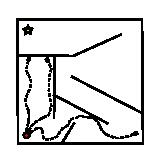
\includegraphics[width=0.55\textwidth]{../Figures/Misc/maze3.eps}
\end{center}
\end{frame}

\begin{frame}{{\scriptsize Evolution of Soft Robots by} Novelty Search}
\begin{center}
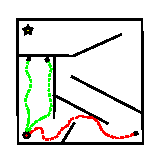
\includegraphics[width=0.55\textwidth]{../Figures/Misc/maze4.eps}
\end{center}
\end{frame}

\begin{frame}{{\scriptsize Evolution of Soft Robots by} Novelty Search}
\begin{block}{What is novelty search:}
\begin{itemize}
\item Traditionally fitness measures how good an individual is.
\item Objective function can prevent evolution reaching the target.
\item Abandon the objective
\item Try finding novelty in behavior space
\end{itemize}
\end{block}
\begin{block}{How to define novelty: Sparsity}
\begin{equation*}
s(x) = \cfrac{1}{k} \sum_{i=0}^k dist(x, b_i)
\end{equation*}
\end{block}
\end{frame}







\section{Related Work}

\begin{frame}{Related Work}
\textit{Evolving virtual creature}s~\footfullcite{sims1994evolving}
\begin{itemize}
\item Rigid body parts, joints
\item Evolution of the morphology and the control
\end{itemize}
{\centering
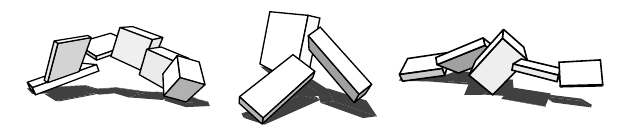
\includegraphics[scale=0.4]{../Figures/Misc/evolvingVirtualCreatures.png}}\\
\textit{Evolving a diversity of virtual creatures through novelty search and local competition} ~\footfullcite{lehman2011evolving}
\begin{itemize}
\item Novelty $<$ Fitness
\item Novelty search with global fitness competition $>$ Fitness
\end{itemize}
\end{frame}

\begin{frame}{Related Work}
\textit{Evolving soft robots with multiple materials and a powerful generative encoding}~\footfullcite{cheney2013unshackling}
\begin{itemize}
\item Generative encoding, Compositional pattern-producing network, CPPN
\item Neuroevolution of augmenting topologies, NEAT
\end{itemize}
\vspace{0.3cm}
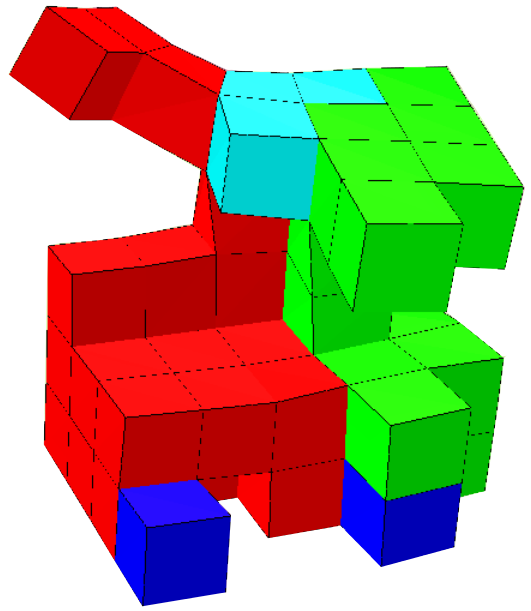
\includegraphics[width=0.3\textwidth,height=0.25\textheight]{../Figures/Misc/unshacklingEvolutionFigure1.png}\	\	\	
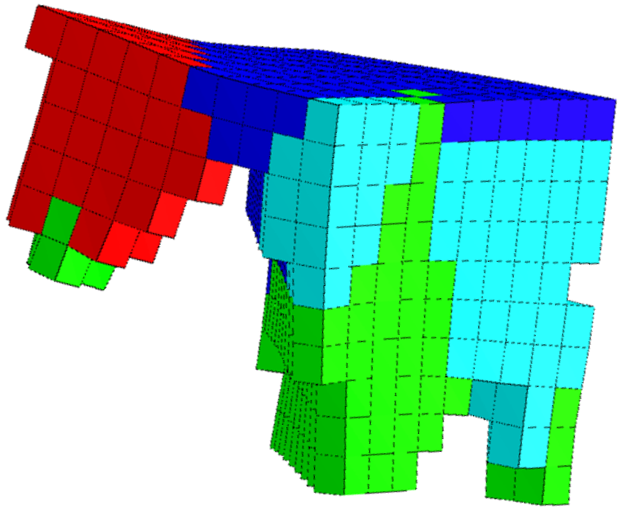
\includegraphics[width=0.3\textwidth,height=0.25\textheight]{../Figures/Misc/unshacklingEvolutionFigure2.png}\	\	\	
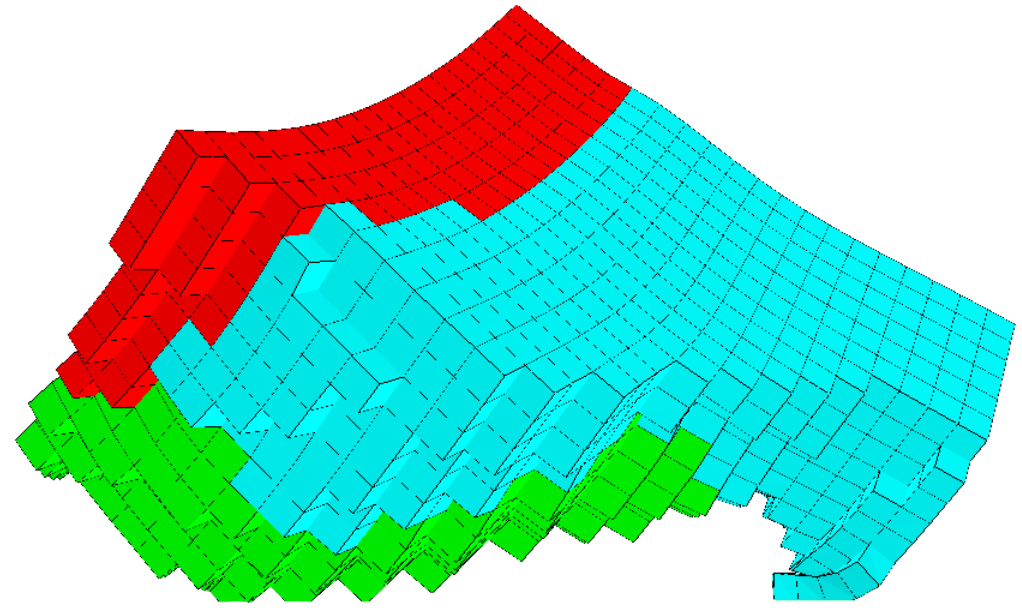
\includegraphics[width=0.3\textwidth,height=0.25\textheight]{../Figures/Misc/unshacklingEvolutionFigure3.png}
\end{frame}









\section{Method}

{
\usebackgroundtemplate{\putat{0}{-275}{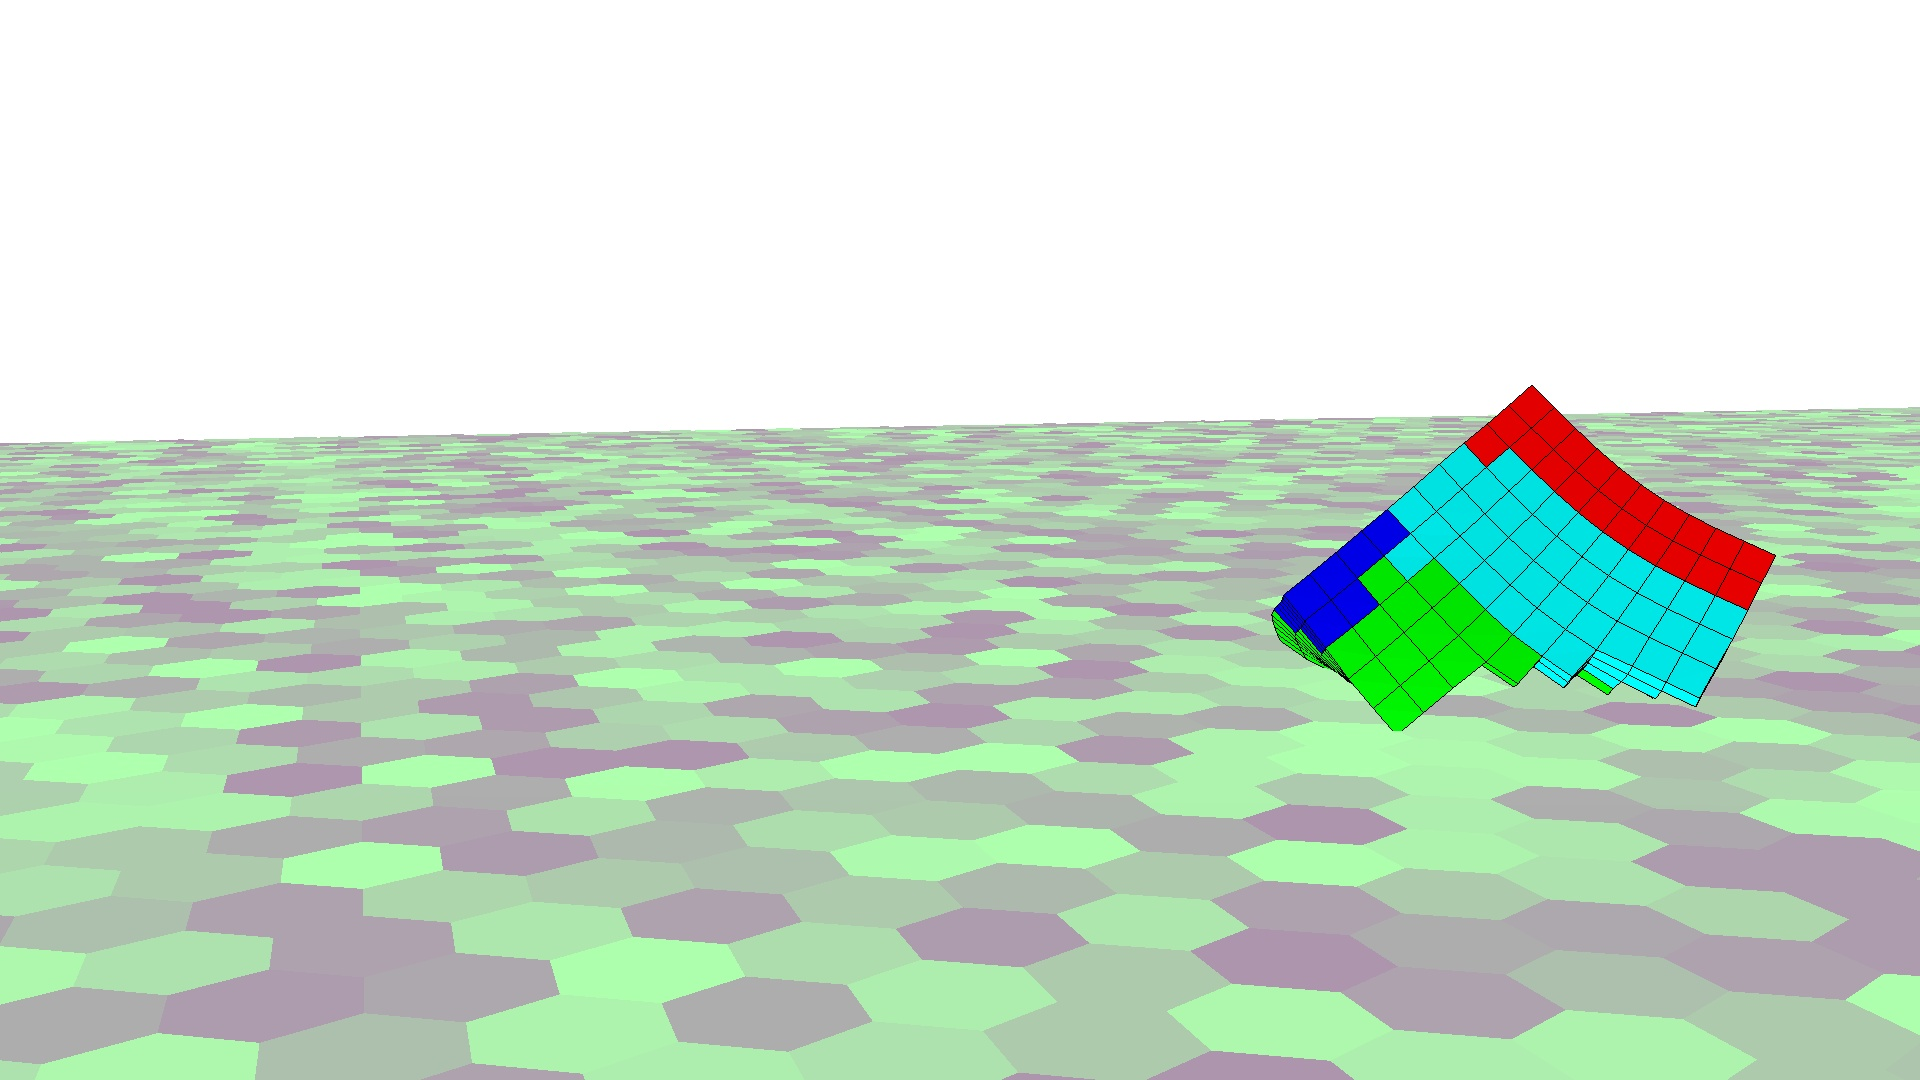
\includegraphics[width=\paperwidth]{../Figures/Misc/000084.jpg}}}
\begin{frame}{Soft Robos in Simulation}
\vspace{-0.5cm}
\begin{block}{
\includegraphics[scale=0.35]{../Figures/Misc/voxcad_logo.png}\	VoxCad Simulator~\footfullcite{hiller2012dynamic}}
\begin{itemize}
\item Created by Jonathan Hiller and Hod Lipson
\item Voxel modeling and analyzing software
\item Physics engine extracted and used for the simulations
\end{itemize}
\end{block}
\begin{itemize}
\item Voxels
\item Materials
\item Temperature
\end{itemize}
Possible solution space:
\begin{itemize}
\item for size $5^3$: \textcolor{red}{$2,3 \times 10^{87}$}
\item for size $10^3$: \textcolor{red}{$9.3 \times 10^{698}$}
\end{itemize}
\end{frame}
}


\begin{comment}
\begin{frame}{Random Soft Robots}
\begin{block}{Random}
Assign materials to voxels in a random fashion
\end{block}
\begin{block}{Generative encoding}
Only two parameters can change in this encoding
\begin{enumerate}
\item The probability of adding a new voxel into the structure
\item The probability that the new voxel introduced will use the same kind of material as its connection
\end{enumerate}
\end{block}
\begin{block}{Random CPPNs}
Evolution with high mutation power and no fitness information
\end{block}
\end{frame}
\end{comment}

\begin{comment}
\begin{frame}{Simple genetic algorithm}
\begin{block}{Representation}
\begin{itemize}
\item Each genome is represented by a stream of real numbers in $[ 0,1 ]$.
\begin{equation*}
\underbrace{01010\ldots011011}_\text{Presence}\ \    \underbrace{10101\ldots110011}_{Material_1} \   \ldots\  \underbrace{00011\ldots111110}_{Material_n}
\end{equation*}
\item The length of this stream is equal to:
\begin{equation*}
l = n \times (m + 1)
\end{equation*}
\end{itemize}
\end{block}
Simple genetic algorithm fails to produce locomotion.
\end{frame}
\end{comment}

\begin{frame}{CPPN-NEAT}
\begin{block}{Evolving CPPNs with NEAT}
\begin{itemize}
\item Each genome is represented by a CPPN
\item This CPPN is queried for each input coordinate to output the existance and the type of the material.
\item NEAT evolves these CPPNs
\end{itemize}
\end{block}
\begin{center}
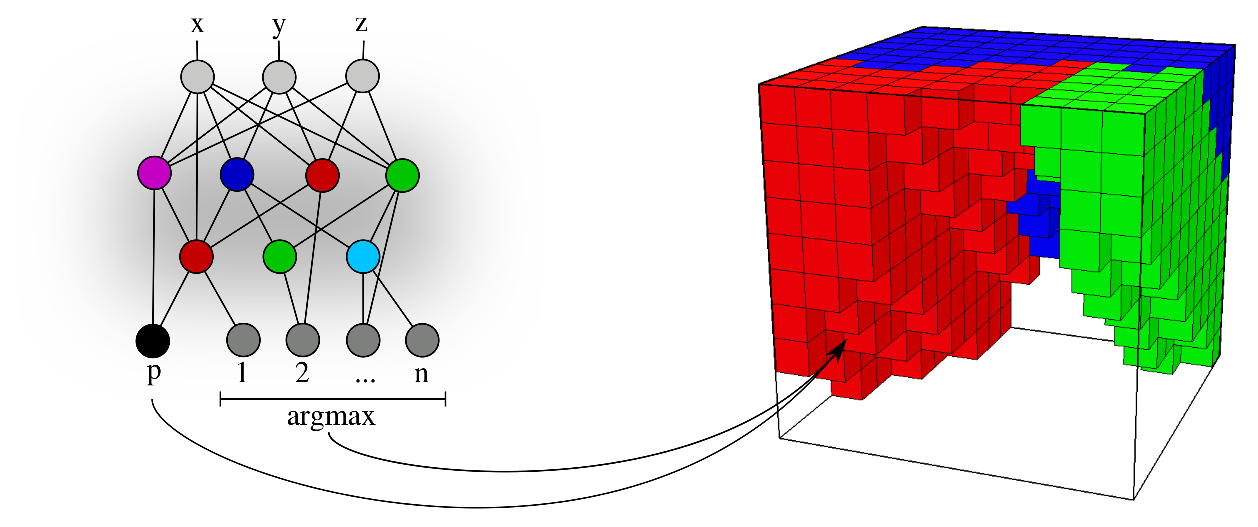
\includegraphics[height=0.4\textheight]{../Figures/Misc/cppnSoftBot2.eps}
\end{center}
\end{frame}

{
\setbeamercolor{block body}{bg=white}

\begin{frame}{Extending CPPN-NEAT with Novelty Search~\footfullcite{lehman2011abandoning}}
\begin{itemize}
\item Novelty takes the place of fitness
\item Novel individuals stored in a list
\item For each new individual in the population, check its novelty in respect to the stored novel individuals.
\end{itemize}
\begin{center}
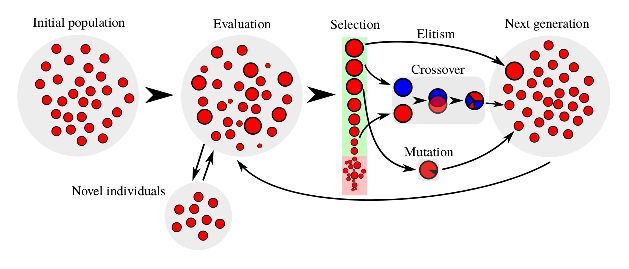
\includegraphics[height=0.45\textheight]{../Figures/Misc/EvolutionNovelty.eps}
\end{center}
\end{frame}

}

\begin{comment}
\begin{frame}{CPPN-NEAT}
\begin{block}{Pseudocode}
\scriptsize
\begin{algorithmic}[1]
\STATE $\mathtt{population} = \varnothing$
\STATE $\mathtt{species} = \varnothing$
\STATE $\mathtt{generation}[0] = \mathbf{initial\_population}()$
\FOR{ $i = 0\   \text{to}\  \mathtt{max\_generation}$}
\STATE $\mathtt{species} = \mathtt{species} \cup \mathbf{speciation}(\mathtt{generation}[i])$
\STATE $\mathbf{evaluation}(\mathtt{generation}[i])$
\STATE $\mathbf{adjust\_fitness}(\mathtt{generation}[i], \mathtt{species})$
\STATE $\mathbf{selection}(\mathtt{generation}[i], \mathtt{species})$
\STATE $\mathtt{generation}[i+1] = \mathbf{reproduction}(\mathtt{generation}[i])$
\STATE $\mathtt{population} = \mathtt{population} \cup \mathtt{generation}[i+1]$
\ENDFOR
\end{algorithmic}
\end{block}
\end{frame}

\begin{frame}{CPPN-NEAT with Novelty Search}
\begin{block}{Pseudocode}
\scriptsize
\begin{algorithmic}[1]
\STATE $\mathtt{population} = \varnothing$
\STATE $\mathtt{novel\_inds} = \varnothing$
\STATE $\mathtt{species} = \varnothing$
\STATE $\mathtt{generation}[0] = \mathbf{initial\_population}()$
\FOR{ $i = 0\   \text{to}\  \mathtt{max\_generation}$}
\STATE $\mathtt{species} = \mathtt{species} \cup \mathbf{speciation}(\mathtt{generation}[i])$
\STATE $\mathbf{evaluation}(\mathtt{generation}[i])$
\FORALL {$\mathtt{ind} \in \mathtt{generation}[i]$}
\STATE $\mathtt{novelty} = \mathbf{sparsity}(\mathtt{ind}, (\mathtt{generation}[i] - \mathtt{ind}) \cup \mathtt{novel\_inds})$
\IF {$(\mathtt{novelty} \geq \mathtt{novelty\_{threshold}}\ ||\ \mathtt{novel\_inds} == \varnothing)$}
\STATE $\mathtt{novel\_inds} = \mathtt{novel\_inds} \cup \mathtt{ind}$
\ENDIF
\ENDFOR
\STATE $\mathbf{adjust\_novelty}(\mathtt{generation}[i], \mathtt{species})$
\STATE $\mathbf{selection}(\mathtt{generation}[i], \mathtt{species})$
\STATE $\mathtt{generation}[i+1] = \mathbf{reproduction}(\mathtt{generation}[i])$
\STATE $\mathtt{population} = \mathtt{population} \cup \mathtt{generation}[i+1]$
\ENDFOR
\end{algorithmic}
\end{block}
\end{frame}

\begin{frame}{CPPN-NEAT with Novelty Search}
\begin{block}{Pseudocode}
\scriptsize
\begin{algorithmic}[1]
\STATE $\mathtt{population} = \varnothing$
\textcolor{red}{
\STATE $\mathtt{novel\_inds} = \varnothing$
}
\STATE $\mathtt{species} = \varnothing$
\STATE $\mathtt{generation}[0] = \mathbf{initial\_population}()$
\FOR{ $i = 0\   \text{to}\  \mathtt{max\_generation}$}
\STATE $\mathtt{species} = \mathtt{species} \cup \mathbf{speciation}(\mathtt{generation}[i])$
\STATE $\mathbf{evaluation}(\mathtt{generation}[i])$
\textcolor{red}{
\FORALL {$\mathtt{ind} \in \mathtt{generation}[i]$}
\STATE $\mathtt{novelty} = \mathbf{sparsity}(\mathtt{ind}, (\mathtt{generation}[i] - \mathtt{ind}) \cup \mathtt{novel\_inds})$
\IF {$(\mathtt{novelty} \geq \mathtt{novelty\_{threshold}}\ ||\ \mathtt{novel\_inds} == \varnothing)$}
\STATE $\mathtt{novel\_inds} = \mathtt{novel\_inds} \cup \mathtt{ind}$
\ENDIF
\ENDFOR
\STATE $\mathbf{adjust\_novelty}(\mathtt{generation}[i], \mathtt{species})$
}
\STATE $\mathbf{selection}(\mathtt{generation}[i], \mathtt{species})$
\STATE $\mathtt{generation}[i+1] = \mathbf{reproduction}(\mathtt{generation}[i])$
\STATE $\mathtt{population} = \mathtt{population} \cup \mathtt{generation}[i+1]$
\ENDFOR
\end{algorithmic}
\end{block}
\end{frame}
\end{comment}

\begin{comment}
{
\setbeamercolor{block body}{bg=white}

\begin{frame}{Behavior}
\begin{block}{For novelty search, behaviors need to be defined}
\vspace{0.2cm}
\begin{center}
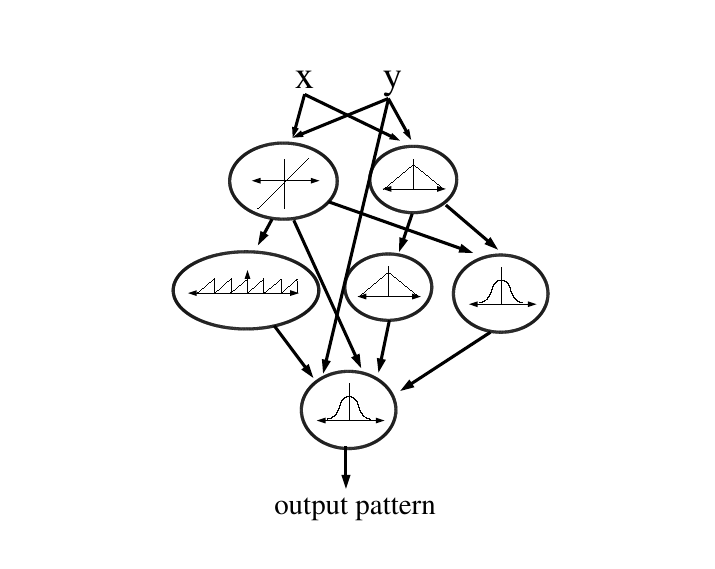
\includegraphics[height=0.15\textheight]{../Figures/Misc/cppnNetwork.png}\	
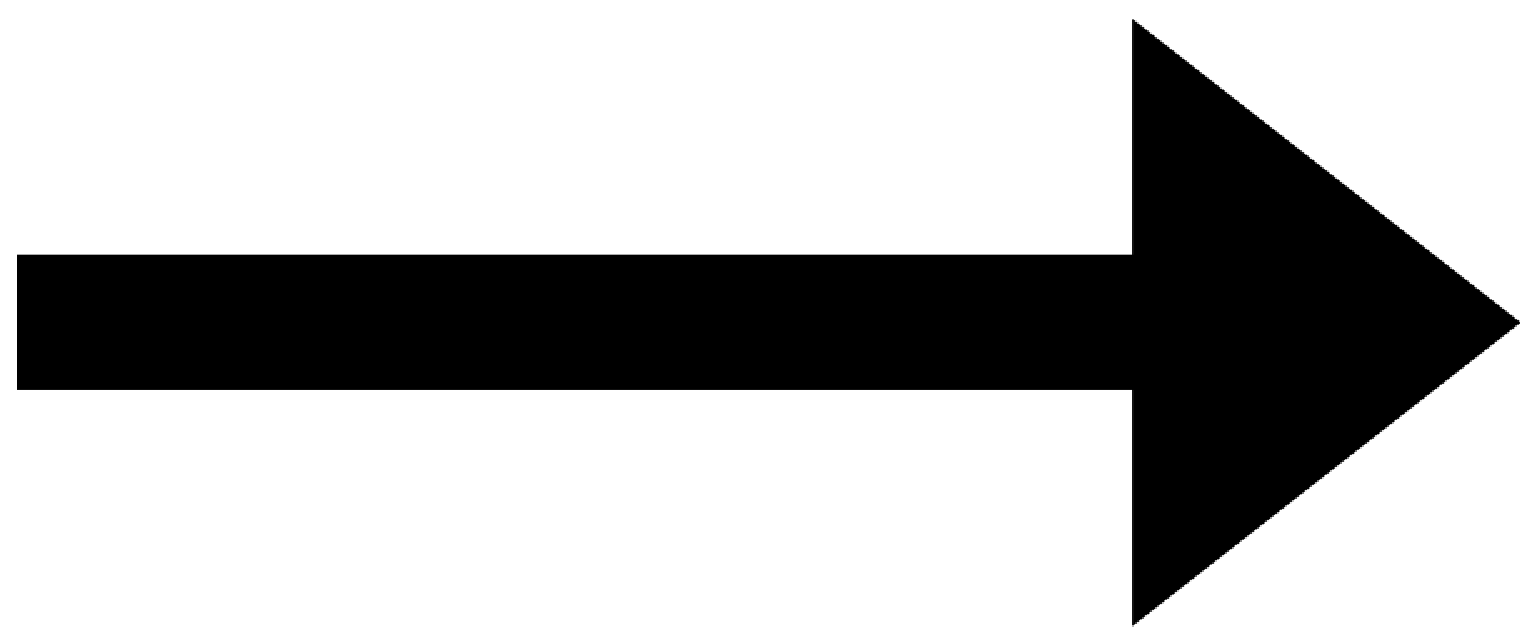
\includegraphics[height=0.05\textheight]{../Figures/Misc/Arrow_east.eps}\	
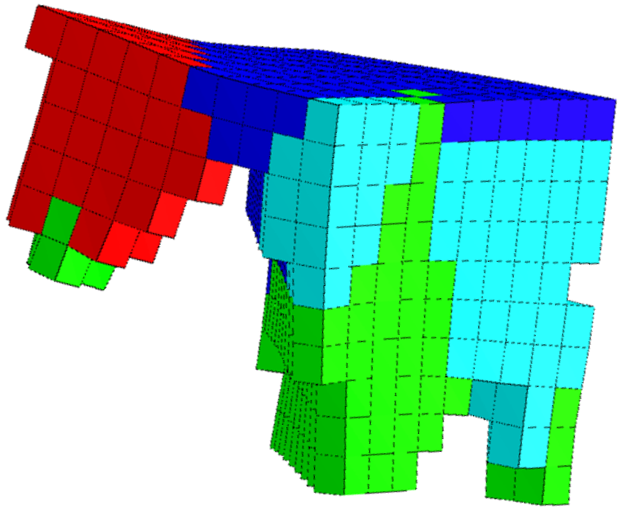
\includegraphics[height=0.15\textheight]{../Figures/Misc/unshacklingEvolutionFigure2.png}\	
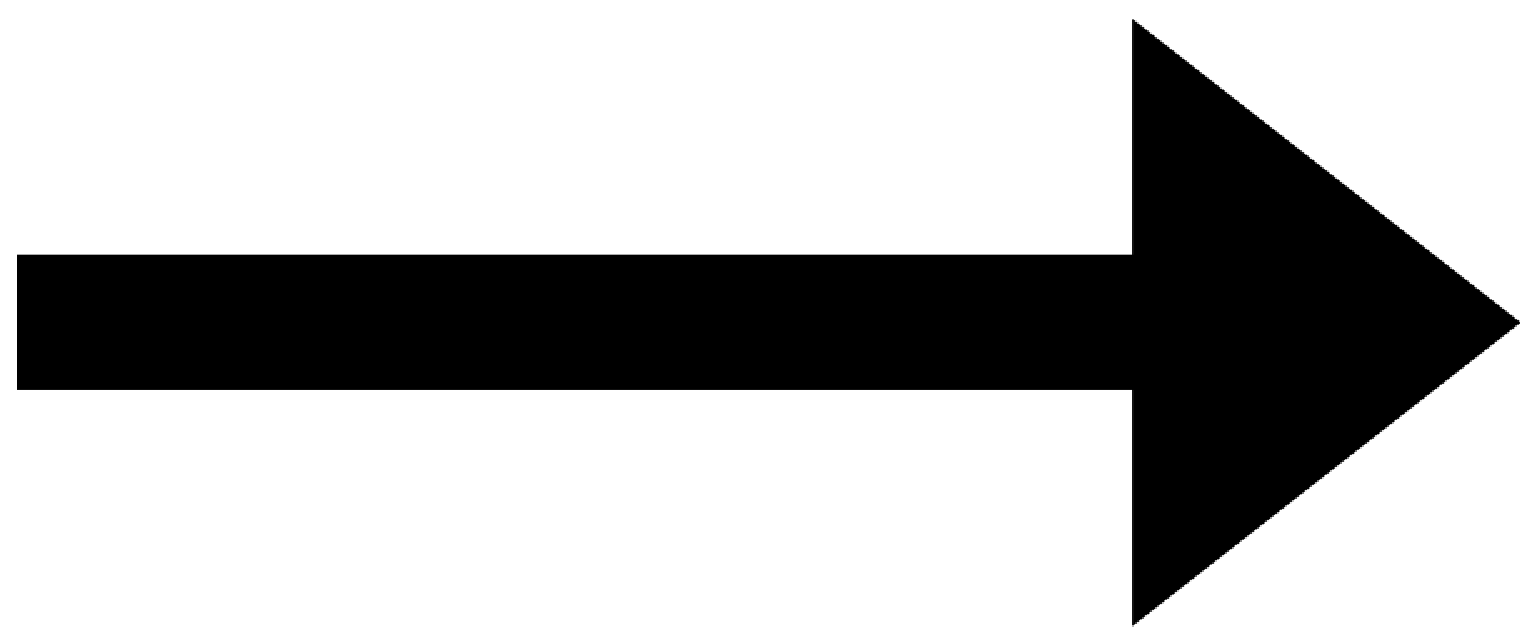
\includegraphics[height=0.05\textheight]{../Figures/Misc/Arrow_east.eps}\	
{\huge $F(x)$ }\	
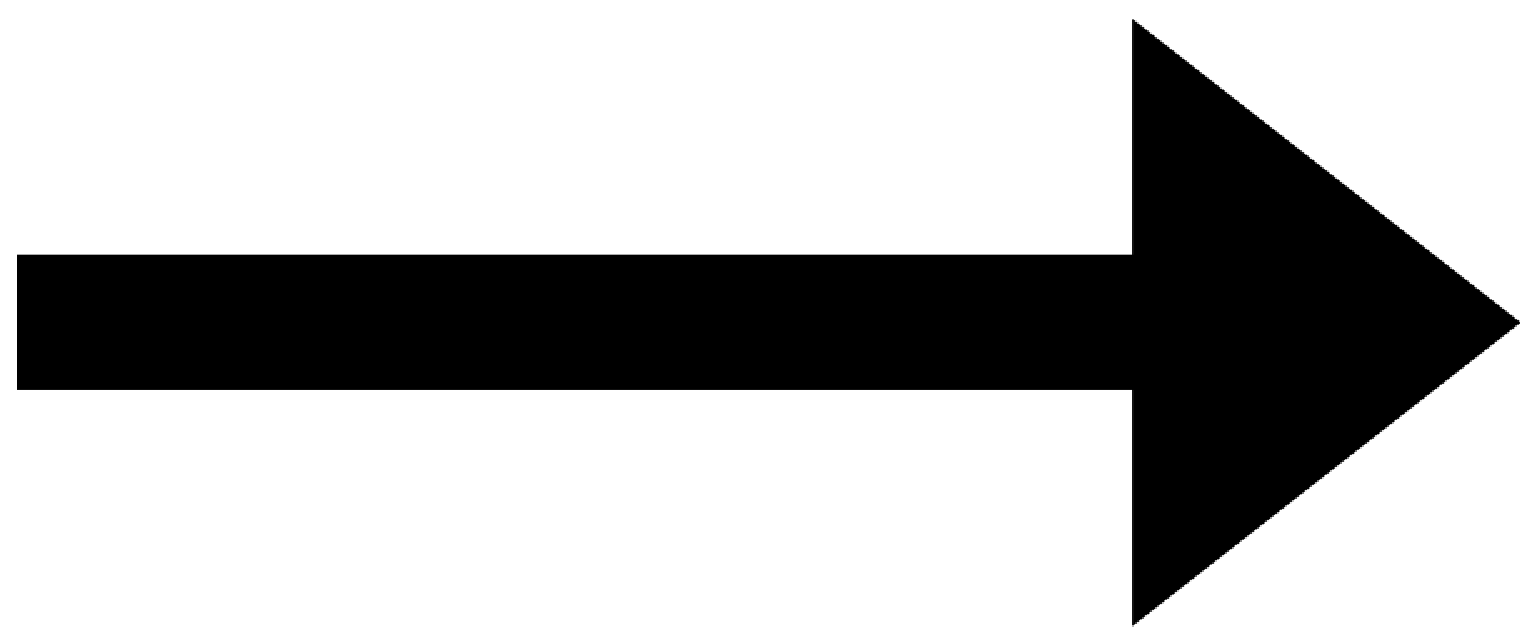
\includegraphics[height=0.05\textheight]{../Figures/Misc/Arrow_east.eps}\	
{\huge $B(x)$ }\\
\end{center}
\end{block}
\end{frame}

}
\end{comment}

\begin{frame}{Behaviors}
\begin{minipage}[t][8cm][b]{0,49\textwidth}
\begin{table}
\centering
    \begin{tabular}{p{1.5cm} c}
    \Vcentre{2D-traj.} &
    \Vcentre{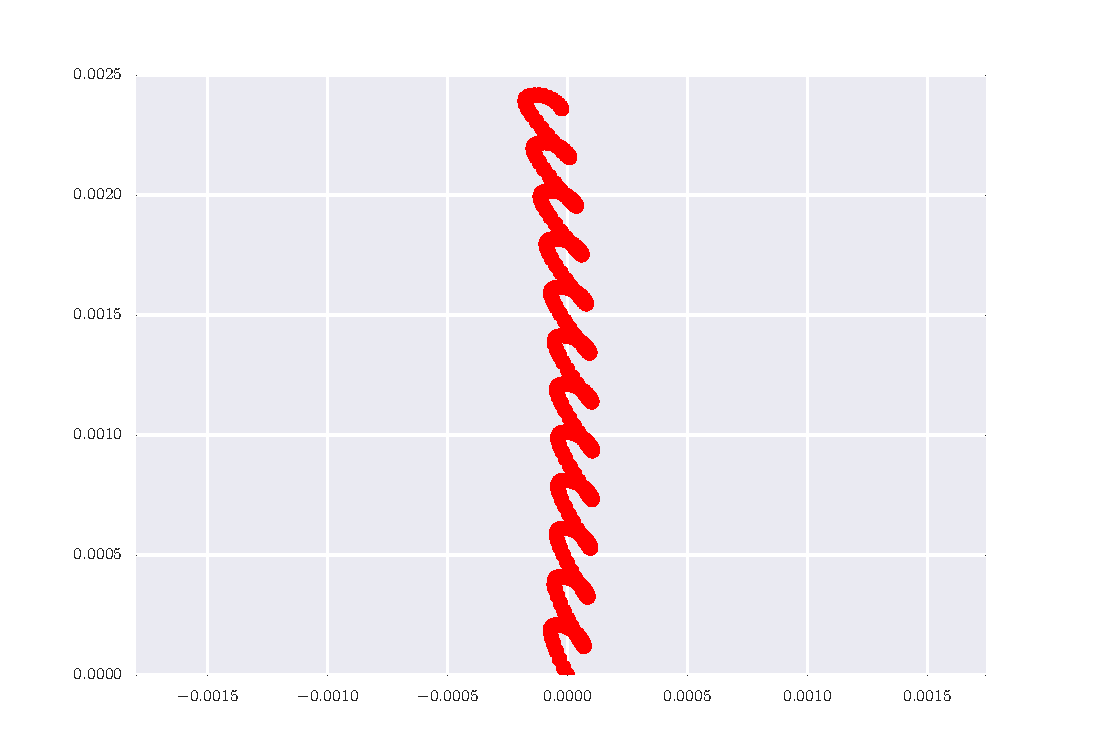
\includegraphics[scale=0.18]{../Figures/Behaviors/2d.pdf}}\\
    \Vcentre{3D-traj.}    &
    \Vcentre{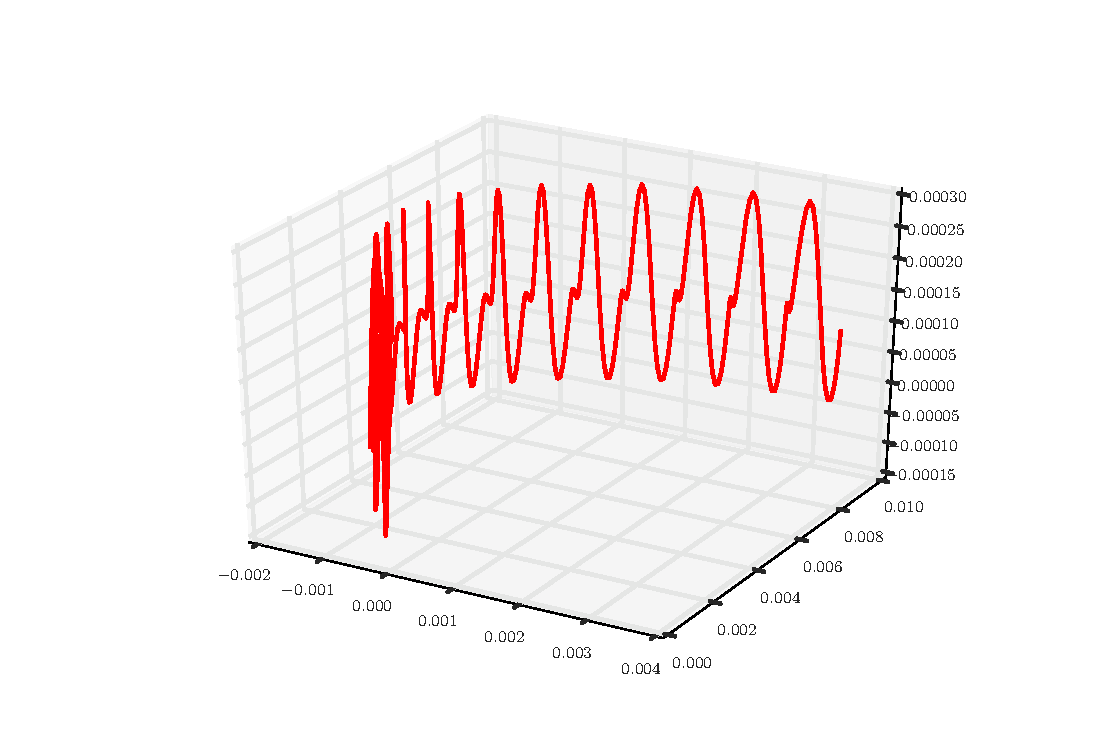
\includegraphics[scale=0.15]{../Figures/Behaviors/3d.pdf}}\\
    \Vcentre{Pace}   &
    \Vcentre{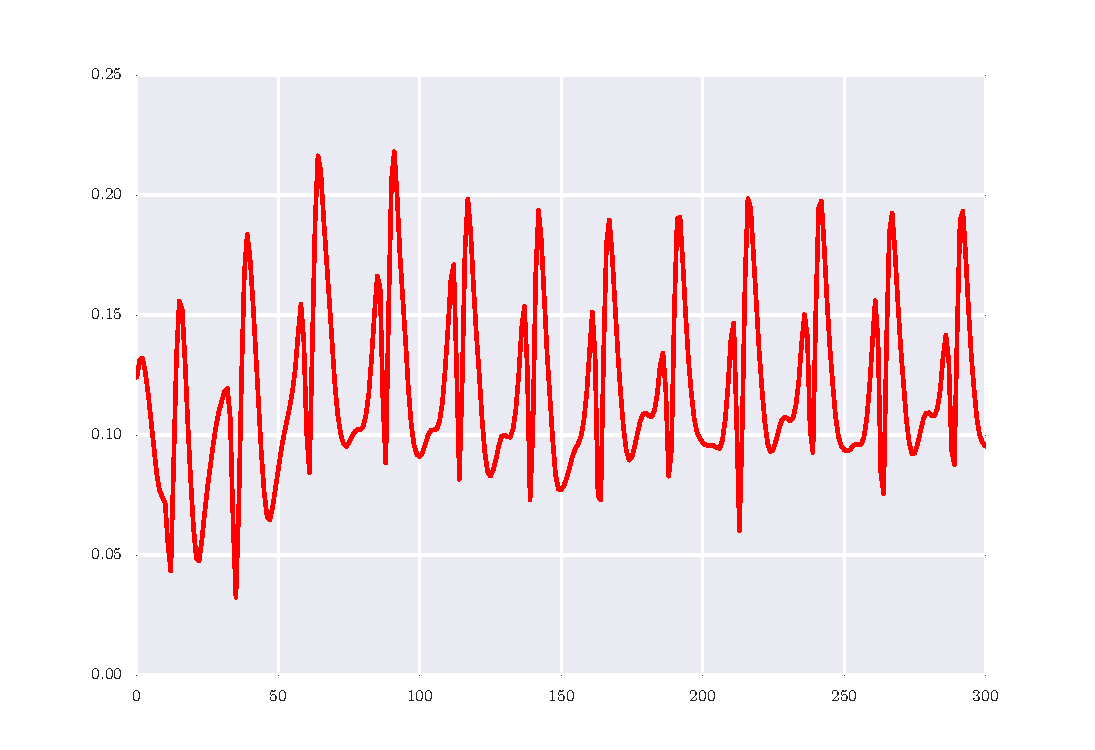
\includegraphics[scale=0.15]{../Figures/Behaviors/pace.pdf}}\\
    \Vcentre{DFT-Pace} &
    \Vcentre{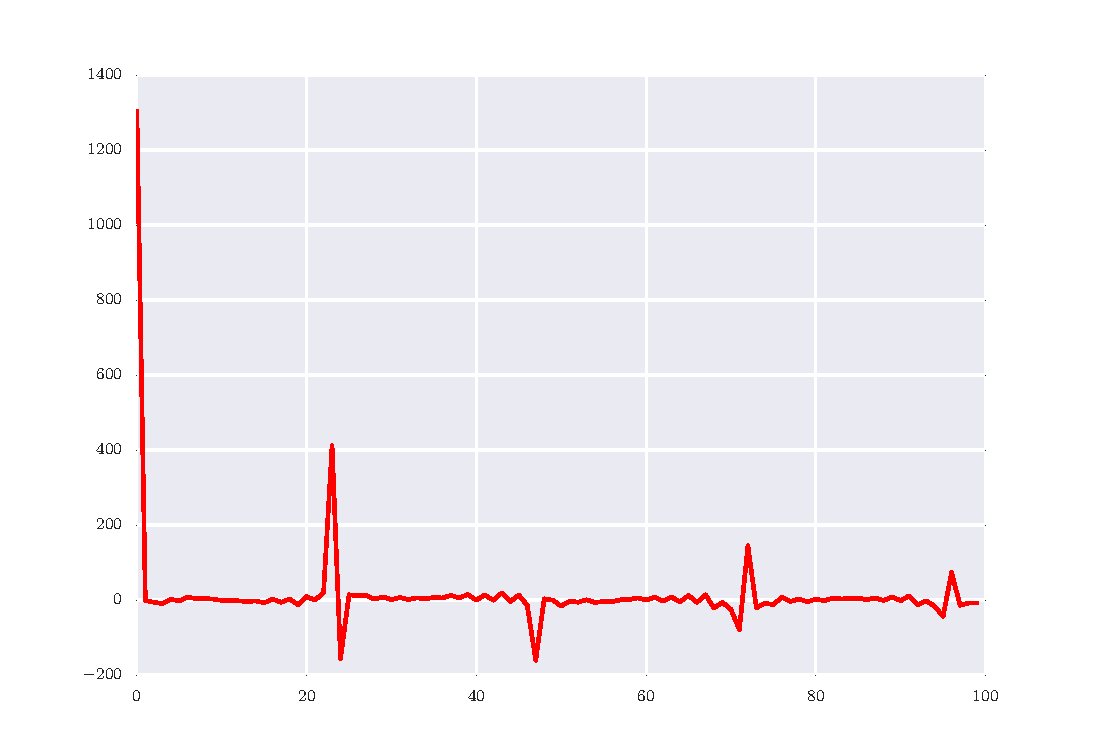
\includegraphics[scale=0.15]{../Figures/Behaviors/pacedft.pdf}}\\
    \end{tabular}
\end{table}
\end{minipage}
\begin{minipage}[t][8cm][b]{0,49\textwidth}
\begin{table}
\centering
    \begin{tabular}{p{1.5cm} c}
    \Vcentre{VTG} &
    \Vcentre{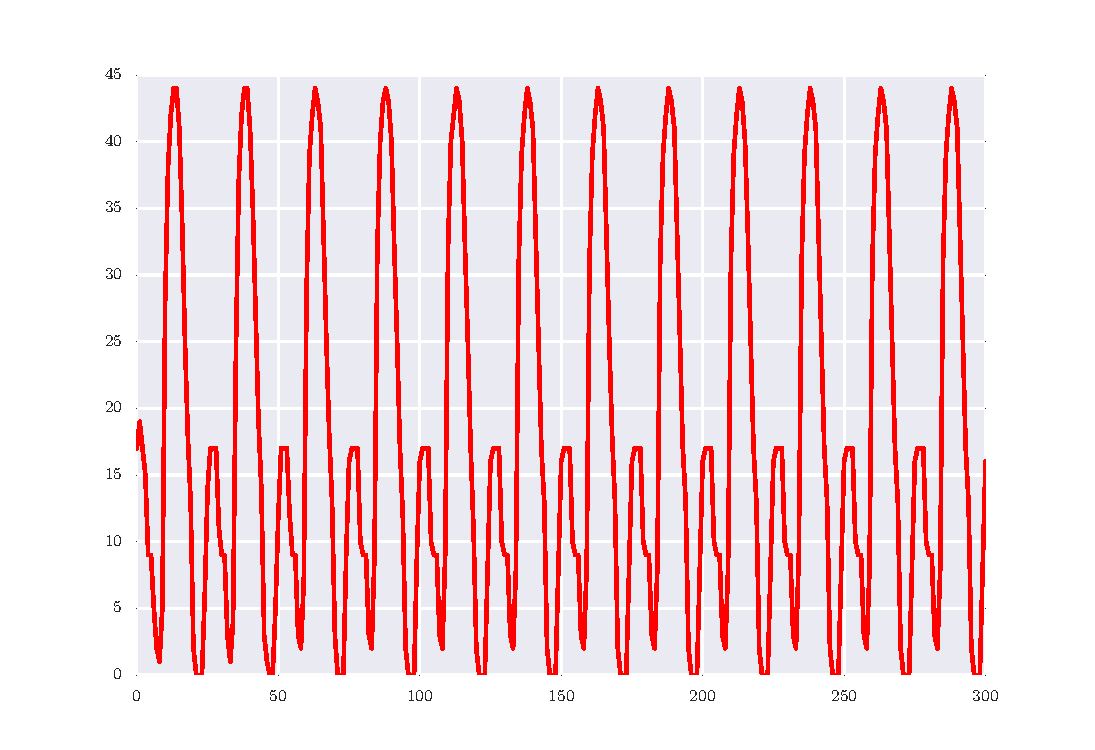
\includegraphics[scale=0.10]{../Figures/Behaviors/vtg.pdf}}\\
    \Vcentre{DFT-VTG}    &
    \Vcentre{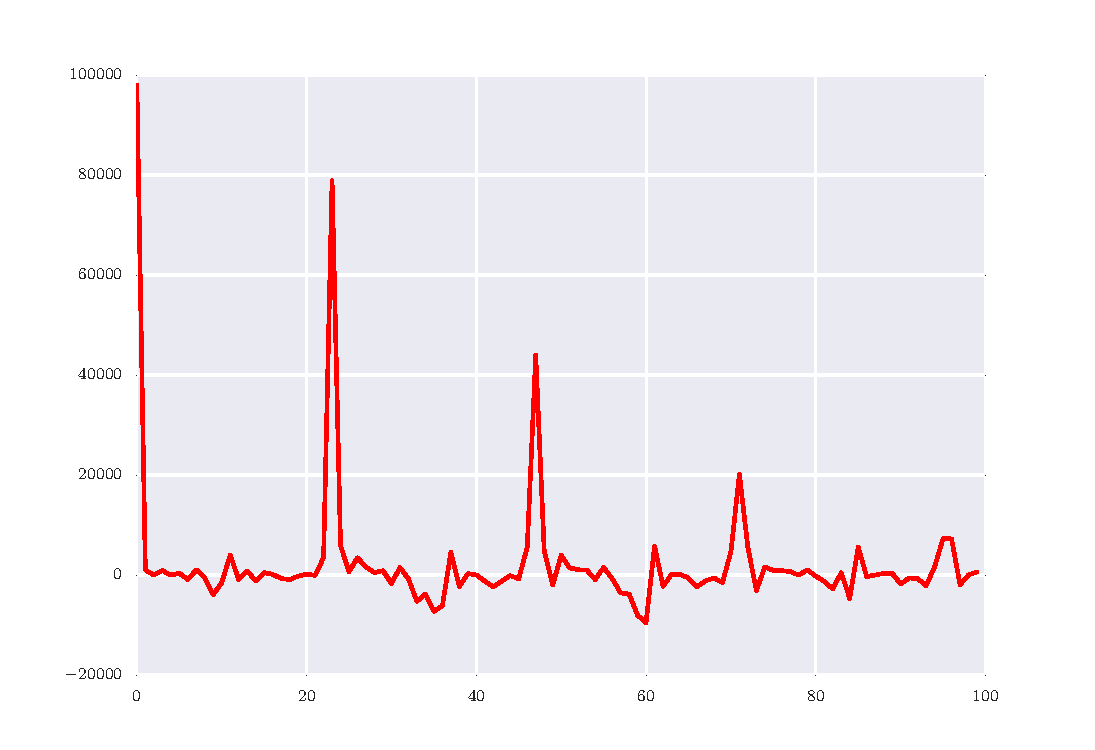
\includegraphics[scale=0.10]{../Figures/Behaviors/vtgdft.pdf}}\\
    \Vcentre{Pr}   &
    \Vcentre{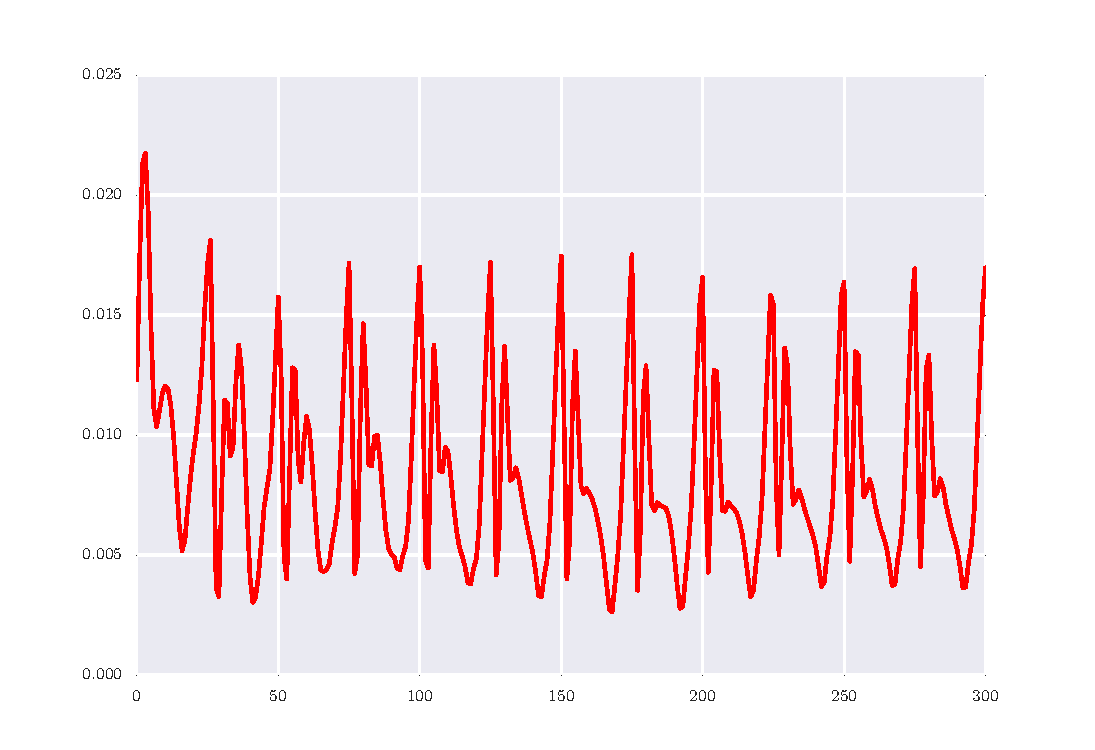
\includegraphics[scale=0.10]{../Figures/Behaviors/pr.pdf}}\\
    \Vcentre{DFT-Pr} &
    \Vcentre{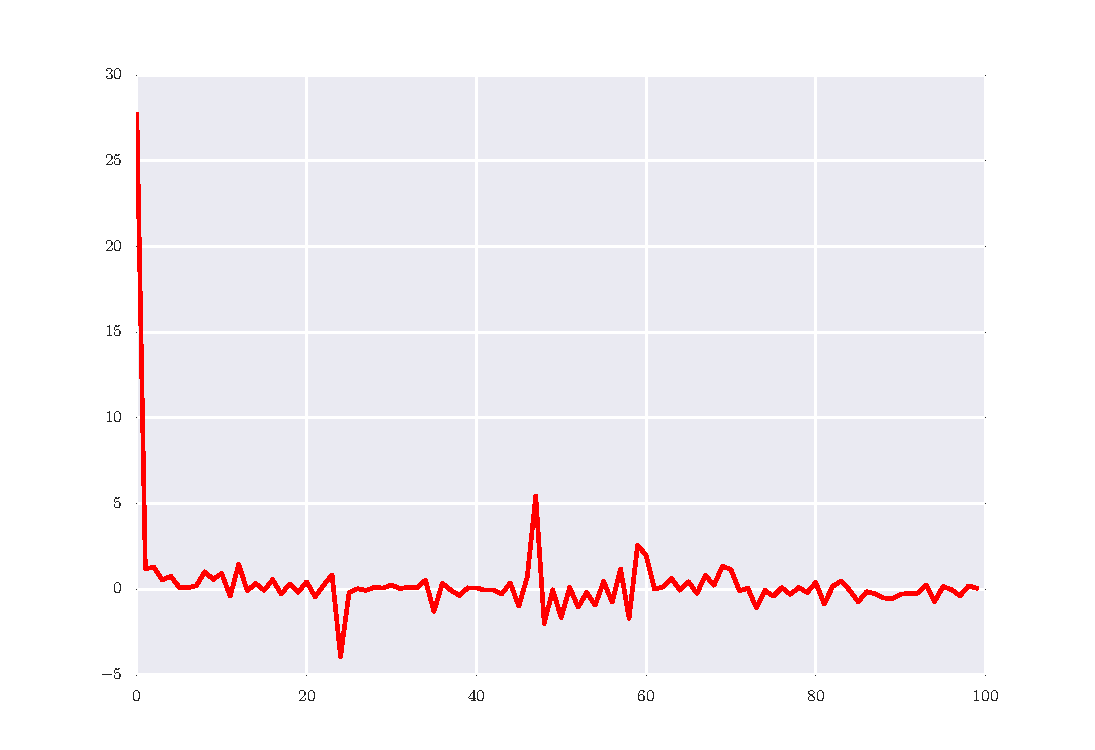
\includegraphics[scale=0.10]{../Figures/Behaviors/prdft.pdf}}\\
    \Vcentre{KE} &
    \Vcentre{\includegraphics[scale=0.10]{../Figures/Behaviors/ke.pdf}}\\
    \Vcentre{DFT-KE} &
    \Vcentre{\includegraphics[scale=0.10]{../Figures/Behaviors/kedft.pdf}}\\
    \end{tabular}
\end{table}
\end{minipage}
\end{frame}


\begin{frame}{Incorporating fitness information into Novelty Search}
\begin{center}
\includegraphics[width=\textwidth]{../Figures/Misc/EvolutionNoveltyFitnessElitism.eps}
\end{center}
\begin{itemize}
\item Keeping properties of novelty search
\end{itemize}
\end{frame}

\begin{comment}
\begin{frame}{Behaviors}
\begin{table}
\centering
    \begin{tabular}{p{3.5cm} c}
    \Vcentre{2D-trajectory} &
    \Vcentre{\includegraphics[scale=0.18]{../Figures/Behaviors/2d.pdf}}\\
    \Vcentre{DFT-Pace}  &
    \Vcentre{\includegraphics[scale=0.18]{../Figures/Behaviors/pacedft.pdf}}\\
    \Vcentre{VTG}                  &
    \Vcentre{1 KHz}     &                     &
    \Vcentre{\includegraphics[scale=0.18]{../Figures/Behaviors/vtg.pdf}}\\
    \Vcentre{DFT-VTG}  &
    \Vcentre{\includegraphics[scale=0.18]{../Figures/Behaviors/vtgdft.pdf}}\\
    \end{tabular}
\end{table}
\end{frame}

\begin{frame}{Behaviors}
\begin{table}
\centering
    \begin{tabular}{p{3.5cm} l c c}
    \Vcentre{Pressure}             &
    \Vcentre{1 KHz}     &                     &
    \Vcentre{\includegraphics[scale=0.18]{../Figures/Behaviors/pr.pdf}}\\
    \Vcentre{DFT-Pressure}         &
    \Vcentre{100 KHz}   &
    \Vcentre{\checkmark}                &
    \Vcentre{\includegraphics[scale=0.18]{../Figures/Behaviors/prdft.pdf}}\\
    \Vcentre{KE}                   &
    \Vcentre{1 KHz}     &                     &
    \Vcentre{\includegraphics[scale=0.18]{../Figures/Behaviors/ke.pdf}}
    \end{tabular}
\end{table}
\end{frame}

\begin{frame}{Behaviors}
\begin{table}
\centering
    \begin{tabular}{p{3.5cm} l c c}
    \Vcentre{DFT-KE}               &
    \Vcentre{100 KHz}   &
    \Vcentre{\checkmark}                &
    \Vcentre{\includegraphics[scale=0.18]{../Figures/Behaviors/kedft.pdf}}\\
    \bottomrule
    \end{tabular}
\end{table}
\end{frame}
\end{comment}

\begin{frame}{Experimental phase}
\begin{block}{Experiments:}
\begin{itemize}
\item For lattice sizes: 5, 7, 10
\item $8$ different behavior metrics
\item $4$ variant gravity, $2$ temp. freq. levels
\item For both fitness, and novelty search
\end{itemize}
\end{block}
\begin{block}{Held at:}
\begin{itemize}
\item 2 $\times$ Servers (16-core \& 8-core)
\item 2 $\times$ Desktops (4-core)
\end{itemize}
\end{block}
\alert{More than 20.000 hours of CPU time (single-core)}
\end{frame}











\section{Results}

{
\setbeamercolor{block body}{bg=white}

\begin{frame}{Increased Diversity}
\begin{block}{Novelty Search - Champions every 100 generations:}
\includegraphics[width=0.2\textwidth]{../Figures/Robots/n_4_g_100.jpg}
\includegraphics[width=0.2\textwidth]{../Figures/Robots/n_4_g_200.jpg}
\includegraphics[width=0.2\textwidth]{../Figures/Robots/n_4_g_300.jpg}
\includegraphics[width=0.2\textwidth]{../Figures/Robots/n_4_g_400.jpg}
\includegraphics[width=0.2\textwidth]{../Figures/Robots/n_4_g_500.jpg}\\
\includegraphics[width=0.2\textwidth]{../Figures/Robots/n_4_g_600.jpg}
\includegraphics[width=0.2\textwidth]{../Figures/Robots/n_4_g_700.jpg}
\includegraphics[width=0.2\textwidth]{../Figures/Robots/n_4_g_800.jpg}
\includegraphics[width=0.2\textwidth]{../Figures/Robots/n_4_g_900.jpg}
\includegraphics[width=0.2\textwidth]{../Figures/Robots/n_4_g_1000.jpg}
\end{block}

\begin{block}{Fitness-based Search - Champions every 100 generations:}
\includegraphics[width=0.2\textwidth]{../Figures/Robots/f_4_g_100.jpg}
\includegraphics[width=0.2\textwidth]{../Figures/Robots/f_4_g_200.jpg}
\includegraphics[width=0.2\textwidth]{../Figures/Robots/f_4_g_300.jpg}
\includegraphics[width=0.2\textwidth]{../Figures/Robots/f_4_g_400.jpg}
\includegraphics[width=0.2\textwidth]{../Figures/Robots/f_4_g_500.jpg}\\
\includegraphics[width=0.2\textwidth]{../Figures/Robots/f_4_g_600.jpg}
\includegraphics[width=0.2\textwidth]{../Figures/Robots/f_4_g_700.jpg}
\includegraphics[width=0.2\textwidth]{../Figures/Robots/f_4_g_800.jpg}
\includegraphics[width=0.2\textwidth]{../Figures/Robots/f_4_g_900.jpg}
\includegraphics[width=0.2\textwidth]{../Figures/Robots/f_4_g_1000.jpg}
\end{block}
\end{frame}

\begin{comment}
\begin{frame}{Increased Performance}
\begin{block}{Best so far fitness, runs: 10, size: $5^3$}
\centering
\includegraphics[width=0.95\textwidth]{../Figures/Results/FitNovRandomDirectSize5.pdf}
\end{block}
\end{frame}
\end{comment}

\begin{frame}{Increased Performance}
\begin{block}{Best so far fitness, runs: 10, size: $10^3$}
\centering
\includegraphics[width=0.95\textwidth]{../Figures/Results/FitvsNovVsDirSize10.pdf}
\end{block}
\end{frame}

\begin{comment}
\begin{frame}{Population Comparison}
\begin{block}{Average fitness of generation, runs: 10, size: $7^3$}
\centering
\includegraphics[width=0.95\textwidth]{../Figures/Results/ViolinPlotsAvgGenFitSize7.pdf}
\end{block}
\end{frame}
\end{comment}

\begin{frame}{Population Comparison}
\begin{block}{Champion fitness of generation, runs: 10, size: $7^3$}
\centering
\includegraphics[width=0.95\textwidth]{../Figures/Results/AvgGenerChampNoveltyFitnessSize7.pdf}
\end{block}
\end{frame}

\begin{frame}{Behavior Selection}
\begin{block}{Champion fitness of each run, runs: 10, size: $7^3$}
\centering
\includegraphics[width=1.0\textwidth]{../Figures/Results/BehaviorsPerformance.pdf}
\end{block}
\end{frame}

\begin{frame}{Fitness Elitism in Novelty Search}
\begin{block}{Best so far fitness, runs: 10, size: $10^3$}
\centering
\includegraphics[width=0.95\textwidth]{../Figures/Results/CopyFitChampions10.pdf}
\end{block}
\end{frame}

}








\section{Conclusion}

\begin{frame}{Conclusion}
\begin{itemize}
\item Novelty search performs better in respect to fitness
\item Performance is not much affected by the behavior metric
\item Fitness elitism improves performance further
\item Co-evolution of materials alongside morphology
\item Develop methods to combine both searches
\end{itemize}
\end{frame}

{
\usebackgroundtemplate{\putat{0}{-275}{\includegraphics[width=\paperwidth]{../Figures/Misc/000084.jpg}}}

\begin{frame}[plain]
\begin{center}
{\Huge Thank you!}
\end{center}
\end{frame}

}

\end{document}
